%!TEX root = ../dissertation.tex

\chapter{Implementation}
\label{chp:implementation}
This chapter describes the practical realization of the Social Media Kit (\textbf{SMKIT}) project. It provides a detailed explanation of how the system was constructed, focusing on its key modules, components, and their integration to automate content generation and sharing across multiple platforms. 

The chapter begins with an overview of the system architecture, highlighting the modular design and data flow through the system. Subsequently, it dig into the specifics of the core modules, schema management, template customization, social media integration, and the utility functions supporting the system's operations. Additionally, the chapter discusses the possible interaction through the command-line interface (\textbf{CLI}), which enables the use of \textbf{SMKIT}. Furthermore, the implementation of the Web Connector for generating HTML web pages is also examined.

Building on the methodology outlined in the previous chapter, this chapter bridges the theoretical framework with the technical implementation, providing a comprehensive view of how \textbf{SMKIT} was developed to achieve its goals.


\section{Introduction}
\label{sec:implementation_introduction}
The implementation chapter examine the technical realization of the \textbf{Social Media Kit (SMKIT)} project, outlining how the system's design was transformed into a functional software tool. The goal of \textbf{SMKIT} is to facilitate the generation and sharing of engaging content across various social media platforms, ensuring consistency, efficiency, and adaptability.

This section provides an overview of the implementation approach, focusing on the integration of key components that enable \textbf{SMKIT} to meet its objectives. Key areas of emphasis include:

\begin{itemize}
    \item \textbf{System Architecture}: Highlighting the modular design that aid the integration of diverse functionalities.
    \item \textbf{Core Components}: Explaining the implementation of the foundational modules—\textbf{Base Module}, \textbf{Generic Module}, and \textbf{Negapedia Module}—which are integral to the system's operation.
    \item \textbf{Interaction Mechanisms}: Discussing the command-line interface (\textbf{CLI}) as the primary method of user interaction with the system.
    \item \textbf{Web Connector Integration}: Detailing the implementation of the Web Connector to generate HTML web pages, expanding the reach of the content beyond social media platforms.
    \item \textbf{Social Media Integration}: Addressing how \textbf{SMKIT} interfaces with platforms like \textbf{Facebook} and \textbf{Twitter} to automate content posting.
    \item \textbf{Utility Modules}: Examining auxiliary functionalities, such as logging, input validation, image processing, and translation management, that support the system's core operations.
\end{itemize}

By systematically detailing these components, this chapter bridges the gap between the conceptual design discussed in the \textbf{Methodology} chapter and the practical application of \textbf{SMKIT}. It provides the reader with a comprehensive understanding of the technical foundation of the project.


\section{System Architecture Overview}
\label{sec:system_architecture_overview}
This section provides a comprehensive overview of the system architecture of \textbf{SMKIT}. It looks into the modular design principles adopted during development and explains how the various components interact to achieve seamless functionality. The section emphasizes the modular approach, which enhances the scalability, maintainability, and adaptability of the system. Additionally, the data flow within the system is detailed to illustrate the end-to-end process of content creation and sharing. A diagram depicting the system architecture and data flow is included to provide visual clarity.

\subsection{Modular Architecture}
\label{subsec:modular_architecture}
The architecture of \textbf{SMKIT} is built on a modular design principle, where each component is implemented as an independent module with a specific responsibility. This design enables the system to be easily extended and maintained. The core modules of \textbf{SMKIT} include:

\begin{itemize}
    \item \textbf{Base Module}: Provides the foundational structure for the system. It serves as an abstract base class, defining common methods and properties, such as:
        \begin{itemize}
            \item Abstract methods for subclass-specific implementations:
                \begin{itemize}
                    \item \texttt{handle\_module()}
                    \item \texttt{process\_pages()}
                    \item \texttt{extract\_pages\_info()}
                \end{itemize}
            \item Static method implemented in-class:
                \begin{itemize}
                    \item \texttt{fetch\_page\_content()}
                \end{itemize}
            \item Shared utilities, including a global color manager for plotting data visualization.
            \item Generating posts through connectors (Facebook, Twitter, Web) using the method \texttt{generate\_posts()}.
        \end{itemize}

    \item \textbf{Generic Module}: Processes data from general websites with structured metadata (e.g., Open Graph tags). Its features include:
        \begin{itemize}
            \item Implements \texttt{process\_pages()} to validate input, fetch page content, and extract metadata into the \texttt{PageInfo} schema.
            \item Supports only the \texttt{summary} mode, processing one page at a time.
        \end{itemize}

    \item \textbf{Negapedia Module}: Specializes in processing Negapedia content, providing:
        \begin{itemize}
            \item Support for multiple modes: \texttt{summary}, \texttt{comparison}, and \texttt{ranking}.
            \item Customizable settings for extraction, such as the number of conflict awards, polemic awards, or social jumps to include.
            \item Extraction of specialized metrics into the \texttt{NegapediaPageInfo} schema, including conflict/polemic awards and historical metrics.
        \end{itemize}

    \item \textbf{Web Connector}: Generates HTML pages with the same content shared on social media, ensuring consistency across platforms.
    \item \textbf{Social Media Connectors}: Integrates with platforms such as \textbf{Facebook} and \textbf{Twitter} for automated posting.
\end{itemize}

\subsection{Data Flow}
\label{subsec:data_flow}
The data flow within \textbf{SMKIT} begins with data extraction from either a general website or a specialized source like Negapedia. The extracted data undergoes several stages of processing, transformation, and structuring before it is used for content generation. The process can be summarized as follows:

\begin{enumerate}
    \item \textbf{Data Validation}: Input parameters, such as URLs, modes, and language settings, are validated to ensure they conform to the requirements of the selected module (\textbf{Generic Module} or \textbf{Negapedia Module}). This step ensures that invalid or incomplete input does not disrupt the workflow.
    \item \textbf{Data Extraction}: Based on the input, data is fetched from the source using the appropriate module. The \textbf{Generic Module} extracts metadata from general websites (e.g., \textbf{Open Graph} tags), while the \textbf{Negapedia Module} retrieves structured data specific to Negapedia.
    \item \textbf{Data Transformation}: Extracted data is organized into predefined schemas, such as \texttt{PageInfo} for general websites and \texttt{NegapediaPageInfo} for Negapedia-specific content. This step ensures that all information is consistently formatted and ready for content generation.
    \item \textbf{Content Generation}: Processed data is dynamically inserted into predefined templates. These templates are customized for different types of output, including social media posts and web pages. This ensures that the generated content aligns with the intended platform's requirements and presentation style.
    \item \textbf{Content Distribution}: The formatted content is either:
    \begin{itemize}
        \item Posted to social media platforms, such as \textbf{Facebook} and \textbf{Twitter}, via the \textbf{Social Media Connectors}.
        \item Used to generate static HTML web pages via the \textbf{Web Connector}, providing a consistent and shareable representation of the content on the web.
    \end{itemize}
\end{enumerate}

Each stage is designed to ensure data integrity, consistency, and adaptability, meeting the specific requirements of the supported platforms. The consistent integration of components in this workflow highlights the versatility and efficiency of the \textbf{SMKIT} system.

\subsection{System Architecture Diagram}
\label{subsec:system_architecture_diagram}
A system architecture diagram is included here to visually represent the relationships between components, the modular structure and the data flow. The diagram illustrate how data is extracted, processed, and shared, providing a clear understanding of the system's operation.
\begin{figure}[ht]
        \centering
        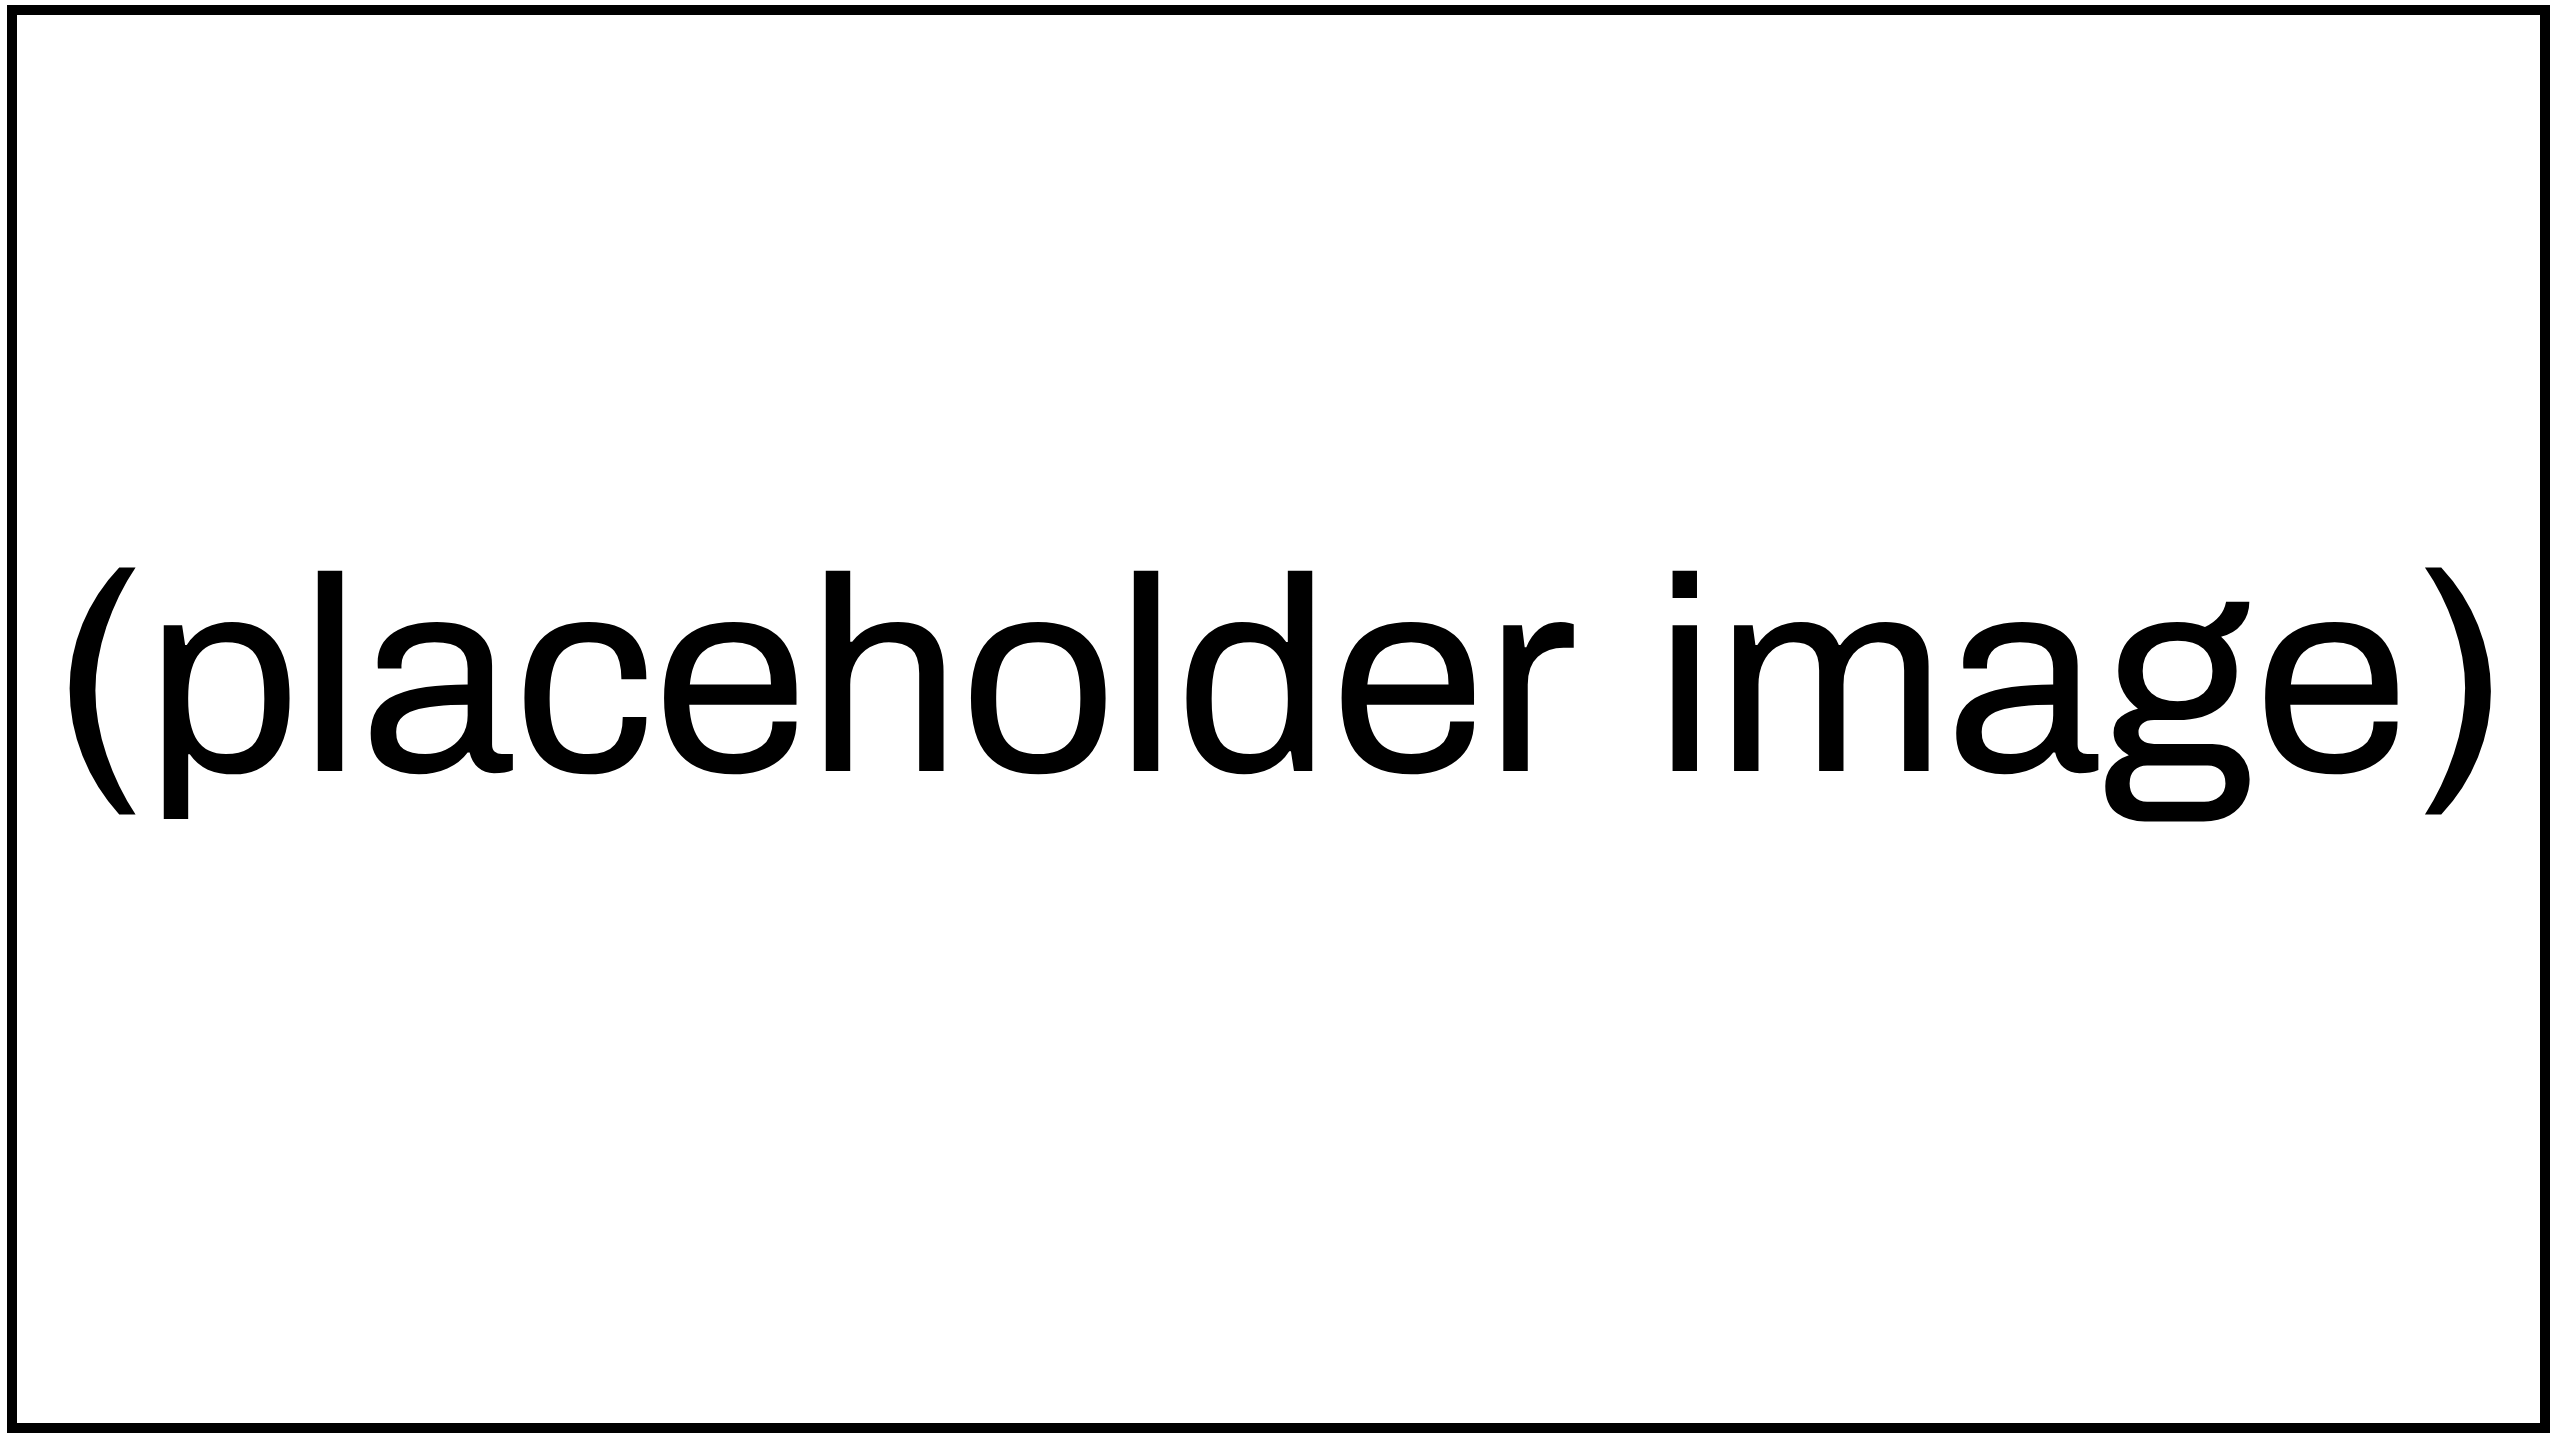
\includegraphics[width=0.8\textwidth]{figures/implementation/placeholder_image.png}
        \caption{System Architecture and Data Flow}
        \label{fig:implementation_system_architecture_and_data_flow}
    \end{figure}


\section{Entry Point and Command-Line Interface (CLI)}
\label{sec:entry_point_and_command_line_interface_cli}

This section describes the main entry point of \textbf{SMKIT}, the \texttt{smkit.py} script, and explains how the system leverages the command-line interface (\textbf{CLI}) to allow users to interact with the tool. The \textbf{CLI} serves as a flexible and efficient means of configuring and executing the system, enabling users to customize operations by specifying input parameters and settings. The \textbf{argparse} library in Python is used to handle command-line arguments, providing a robust mechanism for user input management.

The \texttt{smkit.py} script is the primary entry point for executing \textbf{SMKIT}. It integrates with \textbf{argparse} to define and manage the required and optional arguments that control the behavior of the system. These arguments allow users to specify which module to use, what content to process, and how the output should be generated and distributed.

Key command-line arguments include:

\begin{itemize}
    \item \texttt{--module} (\textit{optional}): Specifies the module to be executed. Supported options include:
    \begin{itemize}
        \item \texttt{generic}: Executes the \textbf{Generic Module} for processing general websites with metadata such as \textbf{Open Graph} tags.
        \item \texttt{negapedia}: Executes the \textbf{Negapedia Module} to process content from Negapedia.
    \end{itemize}
    If not specified, the \textbf{Generic Module} is used by default.

    \item \texttt{--pages} (\textit{mandatory}): A list of page URLs or file paths to be processed. This parameter must be specified for \textbf{SMKIT} to operate. For example:
    \begin{itemize}
        \item \texttt{https://example.com}: Specifies a general website URL for the \textbf{Generic Module}.
        \item \texttt{articles/Donald\_Trump.html}: Specifies a local file path for a Negapedia article to be processed by the \textbf{Negapedia Module}.
    \end{itemize}

    \item \texttt{--mode} (\textit{mandatory}): Specifies the mode of operation for the selected module. Supported modes include:
    \begin{itemize}
        \item \texttt{summary}: Generates a summary for a single page.
        \item \texttt{comparison}: Compares two pages (specific to the \textbf{Negapedia Module}).
        \item \texttt{ranking}: Generates a ranking on selected metrics for pages under analysis (specific to the \textbf{Negapedia Module}).
    \end{itemize}

    \item \texttt{--post\_type} (\textit{mandatory}): Specifies the type of output to generate. Supported options include:
    \begin{itemize}
        \item \texttt{facebook}: Creates posts for \textbf{Facebook}.
        \item \texttt{twitter}: Creates tweets for \textbf{Twitter}.
        \item \texttt{web}: Generates HTML web pages using the \textbf{Web Connector}.
    \end{itemize}
    Multiple options can be selected simultaneously.

    \item \texttt{--message} (\textit{optional}): Provides a custom message for the generated posts. This overrides the default system-generated message.

    \item \texttt{--language} (\textit{optional}, default: \texttt{en}): Specifies the language for the post. Supported options include \texttt{en} (English) and \texttt{it} (Italian).

    \item \texttt{--minimum\_article\_modified\_date} (\textit{optional}): Filters pages based on the last modification date. Pages modified earlier than the specified date (format: \texttt{YYYY-MM-DD}) are ignored.

    \item \texttt{--base\_directory} (\textit{optional}): Specifies the filesystem base directory for local processing. Useful for mapping local files to web URLs.

    \item \texttt{--base\_url} (\textit{optional}): Specifies the base URL of the website for mapping local file paths to accessible web URLs.

    \item \texttt{--remove\_suffix} (\textit{optional}): A flag that, when set, removes \texttt{.html} or \texttt{.htm} suffixes from given paths in \texttt{--pages} parameter values.

    \item \texttt{--number\_of\_words\_that\_matter\_to\_extract} (\textit{optional}): Specifies the number of important words that matter to extract from Negapedia pages.

    \item \texttt{--number\_of\_conflict\_awards\_to\_extract} (\textit{optional}): Specifies the number of conflict awards to extract from Negapedia pages.

    \item \texttt{--number\_of\_polemic\_awards\_to\_extract} (\textit{optional}): Specifies the number of polemic awards to extract from Negapedia pages.

    \item \texttt{--number\_of\_social\_jumps\_to\_extract} (\textit{optional}): Specifies the number of social jumps to extract from Negapedia pages.

    \item \texttt{--ranking\_fields} (\textit{optional}): Specifies the fields to be used for ranking in \texttt{ranking} mode. Supported options include:
    \begin{itemize}
        \item \texttt{recent\_conflict\_levels}
        \item \texttt{recent\_polemic\_levels}
        \item \texttt{mean\_conflict\_level}
        \item \texttt{mean\_polemic\_level}
    \end{itemize}
    If not specified, all ranking fields are used by default.

\end{itemize}

These arguments provide a high degree of flexibility, allowing users to tailor the execution of \textbf{SMKIT} to their specific requirements.


\section{Schema Management and Data Handling}
\label{sec:schema_management_and_data_handling}
This section discusses the schemas used in \textbf{SMKIT} to manage and structure the data effectively. The schemas are central to transforming raw input data into structured formats suitable for content generation and posting on various platforms. Key schemas include \texttt{PageInfo}, \texttt{NegapediaPageInfo}, and \texttt{ImageInfo}, each designed to handle specific aspects of data processing.

\subsection{PageInfo Schema}
\label{subsec:pageinfo_schema}
The \texttt{PageInfo} schema is used for processing general websites, particularly those with metadata such as \textbf{Open Graph} tags. It organizes metadata into a structured format, enabling efficient handling and reuse.

\textbf{Key Fields in the \texttt{PageInfo} Schema:}
\begin{itemize}
    \item \textbf{title}: The title of the page, extracted from the \texttt{og:title} meta tag if available. If not, the HTML \texttt{<title>} tag is used, or the URL as a fallback.
    \item \textbf{description}: A brief description of the page, extracted from the \texttt{og:description} meta tag or the \texttt{name="description"} meta tag as a fallback.
    \item \textbf{message}: A custom message provided by the user as an input parameter. If no custom message is supplied, this field remains \texttt{None}.
    \item \textbf{images}: A list containing information page images, this field will be filled by the primary image of the page, extracted from the \texttt{og:image} meta tag.
    \item \textbf{audio} and \textbf{video}: Links to audio and video content on the page, extracted from the \texttt{og:audio} and \texttt{og:video} meta tags, respectively.
    \item \textbf{urls}: The canonical URL of the page, extracted from the \texttt{og:url} meta tag. If unavailable, the input URL is used.
    \item \textbf{updated\_time}: The timestamp of the last update to the page, extracted from the \texttt{og:updated\_time} meta tag.
    \item \textbf{article\_published\_time} and \textbf{article\_modified\_time}: The publication and modification timestamps of the page, extracted from the \texttt{article:published\_time} together with \texttt{article:modified\_time} meta tags, respectively.
    \item \textbf{article\_tag}: Tag categorizing the article, extracted from the \texttt{article:tag} meta tag.
    \item \textbf{keywords}: Keywords describing the page, extracted from the \texttt{name="Keywords"} meta tag.
\end{itemize}

\textbf{Code Snippet:}
\begin{lstlisting}[language=Python, caption={PageInfo Schema}, label={lst:pageinfo}]
class PageInfo(TypedDict):
    title: Optional[str]
    description: Optional[str]
    message: Optional[str]
    images: List[ImageInfo]
    audio: Optional[str]
    video: Optional[str]
    urls: List[Optional[str]]
    updated_time: Optional[str]
    article_published_time: Optional[str]
    article_modified_time: Optional[str]
    article_tag: Optional[str]
    keywords: Optional[str]
\end{lstlisting}

\subsection{NegapediaPageInfo Schema}
\label{subsec:negapediapageinfo_schema}
The \texttt{NegapediaPageInfo} schema is specifically designed for processing content from Negapedia. It extends the functionality of \textbf{SMKIT} by incorporating fields that are unique to Negapedia’s data, such as conflict levels, polemic levels, awards, and social jumps.

\textbf{Key Fields in the \texttt{NegapediaPageInfo} Schema:}
\begin{itemize}
    \item \textbf{title}: The title of the page, extracted from the \texttt{<title>} HTML element.
    \item \textbf{description}: Currently not populated for Negapedia pages, set to \texttt{None}.
    \item \textbf{message}: A user-provided custom message, if specified during execution.
    \item \textbf{compact\_message}: A generated summary message combining conflict levels, polemic levels, awards, and social jumps.
    \item \textbf{historical\_conflict} and \textbf{historical\_polemic}: Lists of images representing yearly historical conflict and polemic data, visualized as line plots.
    \item \textbf{recent\_conflict\_levels} and \textbf{recent\_polemic\_levels}: Most recent conflict and polemic levels extracted from Negapedia's data.
    \item \textbf{mean\_conflict\_level} and \textbf{mean\_polemic\_level}: Average conflict and polemic levels calculated over the available data.
    \item \textbf{words\_that\_matter}: A list of up to 100 important words associated with the topic, extracted from the \texttt{Word2TFIDF} static variable.
    \item \textbf{conflict\_awards} and \textbf{polemic\_awards}: Awards categorized by conflict and polemic data, such as \textit{Top 1000 of All Time} or \textit{First Place of the Year}.
    \item \textbf{social\_jumps}: A list of significant socially connected topics, with each entry including a title and a link to a related Negapedia article.
\end{itemize}

\textbf{Code Snippet:}
\begin{lstlisting}[language=Python, caption={NegapediaPageInfo Schema}, label={lst:negapediapageinfo}]
class NegapediaPageInfo(TypedDict):
    title: Optional[str]
    description: Optional[str]
    message: Optional[str]
    compact_message: Optional[str]
    historical_conflict: List[ImageInfo]
    historical_polemic: List[ImageInfo]
    historical_conflict_comparison: Optional[List[ImageInfo]]
    historical_polemic_comparison: Optional[List[ImageInfo]]
    recent_conflict_levels: Optional[str]
    recent_polemic_levels: Optional[str]
    mean_conflict_level: Optional[str]
    mean_polemic_level: Optional[str]
    words_that_matter: List[str]
    conflict_awards: Dict[str, List[str]]
    polemic_awards: Dict[str, List[str]]
    social_jumps: List[Dict[str, str]]
\end{lstlisting}

\subsection{ImageInfo Schema}
\label{subsec:imageinfo_schema}
The \texttt{ImageInfo} schema is a supporting schema used within \texttt{PageInfo} and \texttt{NegapediaPageInfo}. It structures information about images, including their dimensions and alt text.

\textbf{Key Fields in the \texttt{ImageInfo} Schema:}
\begin{itemize}
    \item \textbf{image}: Contains the address of the image. This is typically extracted from metadata tags like \texttt{og:image} on web pages or is dynamically generated during visualization in the Negapedia module.
    \item \textbf{image\_width} and \textbf{image\_height}: Represent the dimensions of the image in pixels, often sourced from \texttt{og:image:width} and \texttt{og:image:height} metadata when available.
    \item \textbf{image\_alt}: Stores the alternate text or description of the image, which is either provided by the page metadata (\texttt{og:image:alt}) or generated based on context.
    \item \textbf{location}: Indicates the source location of the image, such as \texttt{"web"} for online images or \texttt{"local"} for dynamically created files.
\end{itemize}

\textbf{Code Snippet:}
\begin{lstlisting}[language=Python, caption={ImageInfo Schema}, label={lst:imageinfo}]
class ImageInfo(TypedDict):
    image: Optional[str]
    image_width: Optional[int]
    image_height: Optional[int]
    image_alt: Optional[str]
    location: Optional[str]
\end{lstlisting}

These schemas work in harmony to handle diverse data sources. The \texttt{PageInfo} schema structures metadata from general websites, while \texttt{NegapediaPageInfo} extends this capability for Negapedia-specific content. The \texttt{ImageInfo} schema ensures consistent handling of image metadata across both. Together, they enable \textbf{SMKIT} to manage data efficiently and generate high-quality content for social media and web platforms.


\section{Core Modules Implementation}
\label{sec:core_modules_implementation}
This section describes the implementation of the core modules in \textbf{SMKIT}. It highlights the modular design and the inheritance relationship between the modules. Specifically, the \textbf{Generic Module} and \textbf{Negapedia Module} extend the \textbf{Base Module}, inheriting its functionality while implementing their specialized behavior.

\subsection{Base Module}
\label{subsec:base_module}
The \textbf{Base Module} is an abstract class that defines the foundational methods and functionality shared by all modules. It employs the \texttt{ABC} module from Python to define abstract methods that must be implemented by derived classes.

\textbf{Methods in the Base Module:}
\begin{itemize}
    \item \textbf{Abstract Methods:}
    \begin{itemize}
        \item \texttt{handle\_module()}: Processes the input arguments and defines the core logic for the module.
        \item \texttt{process\_pages()}: Manages the entire workflow of processing the provided pages.
        \item \texttt{extract\_pages\_info()}: Extracts relevant information from the given URLs.
    \end{itemize}
    \item \textbf{Static Methods:}
    \begin{itemize}
        \item \texttt{fetch\_page\_content()}: Fetches the HTML content of a web page.
    \end{itemize}
    \item \textbf{Implemented Methods:}
    \begin{itemize}
        \item \texttt{generate\_posts()}: Generates posts for the specified platforms.
    \end{itemize}
\end{itemize}

\textbf{Code Snippet:}
\begin{lstlisting}[language=Python, caption={Base Module}, label={lst:base_module}]
class BaseModule(ABC):
    @abstractmethod
    def handle_module(self, args: Any) -> None:
        pass
    
    @abstractmethod
    def process_pages(self, urls: List[str], post_type: List[str], mode: str, remove_suffix: Optional[bool], base_directory: Optional[str], base_url: Optional[str], minimum_article_modified_date: Optional[str], message: Optional[str]) -> None:
        pass
    
    @abstractmethod
    def extract_pages_info(self, urls: List[str], message: Optional[str], mode: str) -> Union[PageInfo, List[NegapediaPageInfo]]:
        pass
    
    @staticmethod
    def fetch_page_content(url: str) -> Optional[str]:
        pass

    def generate_posts(self, post_info: Union[PageInfo, List[NegapediaPageInfo]], post_type: List[str], mode: str) -> None:
        pass
\end{lstlisting}

\subsection{Generic Module}
\label{subsec:generic_module}
The \textbf{Generic Module} extends the \textbf{Base Module} and specializes in handling general websites. It works with pages that use metadata formats like \textbf{Open Graph}.

\textbf{Methods in the Generic Module:}
\begin{itemize}
    \item \textbf{Implemented Methods:}
    \begin{itemize}
        \item \texttt{handle\_module()}: Processes the input arguments and executes the module's logic.
        \item \texttt{process\_pages()}: Manages the entire workflow of processing the provided pages.
        \item \texttt{extract\_pages\_info()}: Extracts relevant information, like title, description, and images, from the given URLs.
    \end{itemize}
\end{itemize}

\textbf{Code Snippet:}
\begin{lstlisting}[language=Python, caption={Generic Module}, label={lst:generic_module}]
class GenericModule(BaseModule):
    def handle_module(self, args: Any) -> None:
        pass
    
    def process_pages(self, urls: List[str], post_type: List[str], mode: str, remove_suffix: Optional[bool], base_directory: Optional[str], base_url: Optional[str], minimum_article_modified_date: Optional[str], message: Optional[str]) -> None:
        pass
    
    def extract_pages_info(self, urls: List[str], message: Optional[str], mode: str) -> PageInfo:
        pass
\end{lstlisting}

\subsection{Negapedia Module}
\label{subsec:negapedia_module}
The \textbf{Negapedia Module} extends the \textbf{Base Module} and is designed specifically to handle content from \textbf{Negapedia}. It implements specialized logic for processing conflict and polemic metrics, as well as generating visual and textual summaries.

\textbf{Methods in the Negapedia Module:}
\begin{itemize}
    \item \textbf{Implemented Methods:}
    \begin{itemize}
        \item \texttt{handle\_module()}: Processes the input arguments and executes the module's logic.
        \item \texttt{process\_pages()}: Processes the input arguments and executes the module's logic.
        \item \texttt{extract\_pages\_info()}: Extracts Negapedia-specific, data such as conflict metrics and awards, from the given URLs..
    \end{itemize}
\end{itemize}

\textbf{Code Snippet:}
\begin{lstlisting}[language=Python, caption={Negapedia Module}, label={lst:negapedia_module}]
class NegapediaModule(BaseModule):
    def handle_module(self, args: Any) -> None:
        pass
    
    def process_pages(self, urls: List[str], post_type: List[str], mode: str, remove_suffix: Optional[bool], base_directory: Optional[str], base_url: Optional[str], minimum_article_modified_date: Optional[str], message: Optional[str]) -> None:
        pass
    
    def extract_pages_info(self, urls: List[str], message: Optional[str], mode: str) -> List[NegapediaPageInfo]:
        pass
\end{lstlisting}


\section{Social Media Integration}
\label{sec:social_media_integration}
This section details the integration of \textbf{SMKIT} with popular social media platforms such as \textbf{Facebook} and \textbf{Twitter}, along with content sharing via \textbf{HTML web pages}. The system automates content distribution by interfacing with APIs and dynamically generating formatted posts.

\subsection{Facebook Connector}
\label{subsec:facebook_connector}
The \textbf{Facebook Connector} integrates \textbf{SMKIT} with the \textbf{Facebook Graph API} for smooth content posting. The main features include:

\begin{itemize}
    \item \textbf{OAuth Authentication:} The system authenticates using \textbf{long-lived page access tokens}. When tokens are expired or missing, it automatically refreshes them through a secure OAuth flow.
    \item \textbf{Content Posting:} Posts are created by loading and customizing templates. Dynamic elements such as titles, descriptions, and images are populated using data from the \texttt{post\_info} structure.
    \item \textbf{Media Upload:} Images are uploaded to Facebook servers before associating them with posts. Both web-hosted and local images are supported.
    \item \textbf{Error Handling:} Robust mechanisms handle token expiration, API errors, and missing data, ensuring the system gracefully responds to failures.
\end{itemize}

The connector supports Facebook-specific formatting requirements and leverages modular functions to process Negapedia data dynamically for \textbf{summary}, \textbf{comparison}, and \textbf{ranking} templates.

\subsection{Twitter Connector}
\label{subsec:twitter_connector}
The \textbf{Twitter Connector} integrates \textbf{SMKIT} with the \textbf{Twitter API} using the \texttt{Tweepy} library. Key capabilities include:

\begin{itemize}
    \item \textbf{OAuth Authentication:} The connector uses access tokens and secret keys for API authentication.
    \item \textbf{Tweet Composition:} Dynamic tweets are generated from templates, with placeholders replaced by specific content such as titles, summaries, and URLs.
    \item \textbf{Media Attachments:} Images are uploaded via Twitter's media API and attached to tweets. The system handles local and web-hosted images with appropriate formatting.
    \item \textbf{Error Handling:} Exceptions during API calls, such as rate-limit violations, are logged to ensure traceability.
\end{itemize}

The connector also adapts content to Twitter-specific requirements such as character limits and media attachment constraints.

\subsection{Unified Social Media Posting}
\label{subsec:unified_social_media_posting}
The \textbf{SMKIT} framework abstracts platform-specific differences, enabling unified content posting across multiple social media channels. The system employs a modular architecture, with connectors for \textbf{Facebook}, \textbf{Twitter}, and additional platforms that can be seamlessly integrated. Key aspects include:

\begin{itemize}
    \item \textbf{Dynamic Routing:} Posts are routed to the appropriate connector based on the specified platform(s).
    \item \textbf{Template Standardization:} Templates are designed to support multiple formats, ensuring consistency across platforms.
    \item \textbf{Scalability:} The architecture supports the addition of new social media platforms with minimal effort by extending the connector framework.
\end{itemize}

\subsection{Web Connector}
\label{subsec:web_connector}
In addition to social media platforms, \textbf{SMKIT} supports content sharing through \textbf{HTML web pages}. The \textbf{Web Connector} generates and formats standalone web pages based on predefined templates. Key features include:

\begin{itemize}
    \item \textbf{Dynamic HTML Generation:} Templates are populated with content from the \texttt{PageInfo} / \texttt{NegapediaPageInfo} structure, including titles, descriptions, images, and links.
    \item \textbf{File Management:} Web pages are saved as standalone HTML files in a user-defined directory.
    \item \textbf{Cross-Platform Compatibility:} HTML pages are designed to be compatible across various devices and browsers, ensuring accessibility.
\end{itemize}

This functionality provides an alternative method of content distribution by enabling users to share URL links to the generated web pages. Additionally, users can host the generated HTML files on their own servers, integrating them as part of their website. These pages can be treated as regular web pages, added to the website's sitemap, and made available for search engine indexing.

\subsection{Error Handling and Reliability}
\label{subsec:error_handling_reliability}
All connectors implement logging and basic error-handling mechanisms to address common issues such as authentication failures, expired tokens, and missing data. The Facebook Connector includes a fallback mechanism for refreshing tokens, while other connectors rely on logging and error reporting. Handling of API rate limits and graceful degradation is limited, emphasizing the need for further enhancements to ensure robust integration across all supported platforms.


\section{Template Management and Customization}
\label{sec:template_management_and_customization}
Templates are an essential part of \textbf{SMKIT}, as they enable dynamic content generation tailored to the requirements of different social media platforms and web pages. This section provides an overview of how templates are managed, customized, and utilized for generating consistent and dynamic content.

\subsection{Template Overview}
\label{subsec:template_overview}
Templates serve as the backbone of \textbf{SMKIT}'s content generation system, providing predefined structures and placeholders for dynamic data insertion. Different templates are designed for \textbf{Facebook}, \textbf{Twitter}, and web posts, each optimized to meet the specific requirements of the target platform.

\begin{itemize}
    \item \textbf{Facebook Templates}: These templates are tailored to Facebook's content layout, supporting features like extended descriptions, embedded images, and optional metadata such as publishing dates or keywords.
    \item \textbf{Twitter Templates}: Optimized for Twitter’s constraints, these templates ensure adherence to character limits and format tweets with concise descriptions and image attachments when available.
    \item \textbf{Web Templates}: These are HTML-based templates used by the \textbf{Web Connector} module to generate static web pages. They are structured to replicate the style and content of social media posts while allowing additional customization options for web use.
\end{itemize}

The system automatically selects the appropriate template based on the \textit{language} and the spread channel in the configuration. This ensures platform-specific optimizations while maintaining consistency across platforms.

\subsection{Template Customization and Data Insertion}
\label{subsec:template_customization_and_data_insertion}
\textbf{SMKIT} dynamically populates templates with data using a systematic approach. Each template contains placeholders for specific fields, which are replaced with content derived from the \texttt{PageInfo} and \texttt{NegapediaPageInfo} schemas. This process ensures smooth integration of dynamic data into preformatted structures.

\begin{itemize}
    \item \textbf{Data Sources}: The schemas provide data such as post titles, descriptions, images, conflict or polemic metrics, and URLs.
    \item \textbf{Dynamic Insertion}: Templates are populated using methods that replace placeholders (e.g., \texttt{\{\{title\}\}}) with actual values. If a placeholder has no corresponding value, the system either removes the line or substitutes it with a default message.
    \item \textbf{Negapedia Integration}: For \textbf{Negapedia} content, the system generates detailed posts based on the selected mode (\texttt{summary}, \texttt{comparison}, or \texttt{ranking}), ensuring tailored and contextually relevant output.
    \item \textbf{Error Handling}: Missing templates or incomplete data trigger logging mechanisms, ensuring errors are reported to the user.
\end{itemize}

This approach enables customization without requiring manual intervention, making the system adaptable to diverse scenarios and content needs, along with easily channel template change over time.

\subsection{Web Connector and Web Page Generation}
\label{subsec:web_connector_and_web_page_generation}
In addition to social media content generation, \textbf{SMKIT} includes functionality for creating static HTML web pages through the \textbf{Web Connector} module. This feature ensures that content shared on social media is also available for web-based distribution.

The web pages generated follow the same structure and content as social media posts, ensuring consistency across platforms. Templates for web pages include placeholders for titles, descriptions, images, and metadata, which are dynamically populated during the generation process.

The \textbf{Web Connector} offers the following capabilities:
\begin{itemize}
    \item \textbf{Generate HTML Pages}: Create static HTML pages using predefined templates that mirror the structure of social media posts.
    \item \textbf{Consistency with Social Media Posts}: Ensure that web pages present identical content to what is shared on social media platforms.
    \item \textbf{Customizable Templates}: Allow users to modify HTML templates to fit specific design styles or branding requirements.
    \item \textbf{Seamless Website Integration}: Enable users to host the generated HTML pages on their own servers, treating them as regular web pages. These pages can be incorporated into their websites' sitemaps, ensuring better discoverability.
    \item \textbf{Easy Sharing}: Provide alternative sharing options through URLs, allowing content to be distributed outside of social media platforms.
\end{itemize}

This functionality enhances the versatility of \textbf{SMKIT}, enabling content creators to maintain a consistent presence across social media and web platforms while offering flexible customization options.


\section{Utility Functions and Support Modules}
\label{sec:utility_functions_and_support_modules}
\textbf{SMKIT} relies on various utility functions and support modules to handle tasks such as input validation, environment configuration, image processing, and logging. These modules are designed to simplify operations, ensure robustness, and facilitate customization.

\subsection{Environment Management}
\label{subsec:Environment_management}
The \textbf{env\_management} module is responsible for securely managing configuration settings, such as API keys, file paths, and other environment variables. This module ensures that sensitive information is loaded from and stored in an environment file (e.g., \texttt{env.json}). Key features include:
\begin{itemize}
    \item \textbf{Secure Storage}: Configuration data is stored in a JSON file.
    \item \textbf{Dynamic Loading}: The \texttt{load\_from\_env} function reads and parses the environment file into memory, allowing modules to access configuration settings seamlessly.
    \item \textbf{Error Handling}: The system gracefully handles missing or corrupted environment files, logging errors to the users.
    \item \textbf{Data Persistence}: The \texttt{save\_to\_env} function updates the environment file with new or modified settings.
\end{itemize}

\subsection{Input Validation Management}
\label{subsec:input_validation_management}
The \textbf{input\_validation\_management} module ensures that user-provided inputs are valid before processing. It verifies input formats, checks for missing fields, and validates URLs or file paths. Key capabilities include:
\begin{itemize}
    \item \textbf{URL Validation}: Identifies and processes valid URLs, distinguishing them from local file paths.
    \item \textbf{File Path Mapping}: Converts local file paths to web-accessible URLs by mapping them based on configured base directories and URLs.
    \item \textbf{Directory Traversal}: Scans directories for files to process, ensuring only supported formats (e.g., HTML, compressed files) are considered.
    \item \textbf{Error Handling}: Invalid inputs trigger detailed error messages and logging, ensuring issues are promptly addressed.
\end{itemize}

\subsection{Image Management}
\label{subsec:image_management}
The \textbf{image\_management} module handles image retrieval and preparation for posting on social media platforms. It ensures images comply with platform-specific requirements. The module’s functionalities include:
\begin{itemize}
    \item \textbf{Image Downloading}: Fetches images from provided URLs using the \texttt{fetch\_image\_as\_stream} function.
    \item \textbf{Format Adaptation}: Adjusts images formats for compatibility with platform constraints.
    \item \textbf{Temporary Storage}: Saves processed images in a designated directory for easy retrieval and posting.
\end{itemize}

\subsection{Logger Management}
\label{subsec:logger_management}
The \textbf{logger\_management} module ensures detailed logging of system activities, including successful operations, warnings, and errors. This facilitates troubleshooting and monitoring. Key aspects include:
\begin{itemize}
    \item \textbf{Custom Logging Format}: Uses a colored formatter for easy differentiation of log levels.
    \item \textbf{Debugging Support}: Provides verbose logs during development to assist in identifying issues.
    \item \textbf{Error Tracking}: Logs errors with detailed context to help pinpoint root causes.
\end{itemize}

\subsection{Plot Colors Management}
\label{subsec:plot_colors_management}
The \textbf{plot\_colors\_management} module manages color schemes for visualizations, ensuring consistency and customization in graphs representing metrics like conflict or polemic levels. Features include:
\begin{itemize}
    \item \textbf{Predefined Color Palette}: A curated list of colors is used to ensure visual consistency across different plots.
    \item \textbf{Dynamic Assignment}: Automatically assigns colors to topics, cycling through the palette or generating new colors if the palette is exhausted.
    \item \textbf{Customization}: Users can modify the color palette to align with branding or specific visualization needs.
\end{itemize}

\subsection{Translation Management}
\label{subsec:translation_management}
The \textbf{translation\_management} module enables multilingual support, allowing \textbf{SMKIT} to generate content in various languages based on user preferences. Its functionalities include:
\begin{itemize}
    \item \textbf{Language-Specific Templates}: Provides localized versions of templates for social media posts and web pages.
    \item \textbf{Fallback Mechanisms}: Falls back to English translations if a specific language translation is unavailable, ensuring uninterrupted operations.
    \item \textbf{Dynamic Placeholder Replacement}: Populates translation strings with dynamic data using placeholders, allowing flexible message customization.
    \item \textbf{Error Handling}: Logs missing translations and warns users of potential content gaps.
\end{itemize}


\section{Conclusion}
\label{sec:implementation_conclusion}
This section summarizes the key aspects of the \textbf{SMKIT} implementation, reflecting on the design choices and technical challenges. It provides a transition to the next chapter, which will discuss the \textbf{Results} of using \textbf{SMKIT} in real-world scenarios.
